%!TEX root = thesis.tex

\chapter{Bayesian aggregation of Galaxy Zoo classifications with SWAP}
\label{chap:1}


\section{This chapter could be about SWAP and incorporate Appendix A}



%%----------------------------------------------------------------------------------------------------------------------------------------------------
%%   Galaxy Zoo 2 Data Description
%%---------------------------------------------------------------------------------------------------------------------------------------------------
\section{Galaxy Zoo 2 Classification Data} \label{sec: data}

Our simulations utilize original classifications made by volunteers during the
 GZ2 project. These data\footnote{\url{data.galaxyzoo.org}} are described in detail
 in~\cite{Willett2013}, though we provide a brief overview here.  The GZ2 subject sample
 consists of 285,962 galaxies identified as the brightest 25\% ($r$-band magnitude $< 17$)
 residing in the SDSS North Galactic Cap region from Data Release 7 and included 
subjects with both spectroscopic and photometric redshifts out to $z < 0.25$.
Subjects were shown as colour composite images via a web-based
 interface\footnote{\url{www.galaxyzoo.org}} wherein volunteers answered a 
series of questions pertaining to the morphology of the subject. With the exception 
of the first question, subsequent queries were dependent on volunteer responses 
from the previous task creating a complex decision tree\added{\footnote{A visualization of this decision tree can be found at \url{https://data.galaxyzoo.org/gz_trees/gz_trees.html}}}. Using GZ2 nomenclature, 
 a \textit{classification} is the total amount of information about a subject 
obtained by completing all tasks in the decision tree. A subject is \textit{retired} 
after it has achieved a sufficient number of classifications.
%\footnote{\url{zoo2.galaxyzoo.org}}


For our current analysis, we choose the first task in the tree: ``Is the galaxy simply 
smooth and rounded, with no sign of a disk?" to which possible responses include 
``smooth", ``features or disk", or ``star or artifact". This \added{choice} serves 
two purposes: 1) this is one of only two questions in the GZ2 decision tree that 
is asked of every subject thus maximizing the amount of data we have to work with, 
and 2) our analysis assumes a binary task and this question is simple enough to cast as such.
 \added{Specifically, we combine ``star or artifact" responses with ``features or disk" responses.}

\replaced{
By combining the ``star or artifact" vote fraction, $f_{artifact}$, with the ``features or disk" vote fraction, $f_{features}$ we obtain a binary response. Here, a vote fraction is simply the fraction of volunteers who voted for a particular response.  We define a label for each GZ2 subject as the majority vote fraction, that is, if \ffeat+\fstar~$ >$ \fsmooth, the galaxy is labelled~\feat, otherwise it is labelled~\notfeat.}
{We assign each subject a descriptive label in order to compare our classification output with GZ2. GZ2 classifications are composed of volunteer vote fractions for each response to every task in the decision tree, denoted as $f_{\mathrm{response}}$. They are derived from the fraction of volunteers who voted for a particular response and are thus approximately continuous. A common technique is to place a threshold on these vote fractions to select samples with an emphasis on purity or completeness, depending on the science case. For our current analysis we choose a threshold of 0.5, that is, if \ffeat+\fstar~$ >$ \fsmooth, the galaxy is labelled~\feat, otherwise it is labelled~\notfeat.  Though naive, we will demonstrate that this threshold produces adequate results, though a more sophisticated mechanism will be explored in a future publication.} 
 We note that only 512 subjects in the GZ2 catalogue have a majority \fstar, contributing less than half a percent contamination \added{by combining the ``star or artifact" with ``features or disk" responses}.

%We note that this threshold is not much different from the suggested 0.430 threshold in \cite{Willett2013} that produces a well-sampled subset of~\feat~galaxies.
The GZ2 catalogue \replaced{assigns every subject three types  of volunteer vote fractions: }{publishes three types of vote fractions for each subject:} raw, weighted, and debiased. Debiased vote fractions are calculated to correct for redshift bias, a task that GZX does not perform. The weighted vote fractions account for inconsistent volunteers.\deleted{, a task we perform as well.} \replaced{However, because our mechanism is entirely different from GZ2,}{The SWAP algorithm (described below) also has a mechanism to weight volunteer votes, however, the two methods are in stark contrast. For consistency,} we derive labels from the raw vote fractions (\raw) \added{that have received no post-processing whatsoever.} In total, the data consist of over 16 million classifications from 83,943 individual volunteers. 


%%----------------------------------------------------------------------------------------------------------------------------------------------------
%%   Talk About SWAP 
%%----------------------------------------------------------------------------------------------------------------------------------------------------
\section{Efficiency through intelligent human-vote aggregation}\label{sec: SWAP}

Galaxy Zoo 2 had a brute-force subject retirement rule whereby each galaxy was to 
receive approximately forty independent classifications.  Once the project reached 
completion, inconsistent volunteers were down-weighted~\citep{Willett2013}, 
a process that does not make efficient use of those who are exceptionally skilled. 
To intelligently manage subject retirement and increase classification efficiency, 
we adapt an algorithm from the Zooniverse  project Space Warps~\citep{Marshall2016}, 
which searched for and discovered several gravitational lens candidates in the 
CFHT Legacy Survey~\citep{More2016}.  Dubbed SWAP (Space Warps Analysis Pipeline), 
 this algorithm computed the probability that an image contained a gravitational lens 
given volunteers' classifications and experience after being shown a training sample 
consisting of simulated lensing events.  We provide a brief overview here.  

The algorithm assigns each volunteer an \textit{agent} which interprets that 
volunteer's classifications. Each agent assigns a 2$\times$2 confusion matrix 
to their volunteer which encodes that volunteer's probability of correctly 
identify feature \A~given that the subject \deleted{actually}exhibits feature \A; 
and the probability of correctly identifying the absence of feature 
\A~\added{(denoted \N)} given that the subject does not exhibit that feature. 
The agent updates these probabilities by estimating them as 

\begin{equation}
P(``X" | X, \mathbf{d}) \approx \frac{\mathcal{N}_{``X"}}{\mathcal{N}_{X}}
\end{equation}
\added{where $X$ is the true classification of the subject and ``$X$" is the classification made by the volunteer upon viewing the subject. Thus} $\mathcal{N}_{``X"}$ is the number of classifications the volunteer labelled as type $X$, 
$\mathcal{N}_X$ is the number of subjects the volunteer has seen that were actually of type $X$,
and $\mathbf{d}$ represents the history of the volunteer, i.e., all subjects they have seen.
\added{Therefore the confusion matrix for a single volunteer goes as}

\begin{eqnarray}
\mathcal{M} & = & \left[
	\begin{array}{cc}
		P(``A"|N, \mathbf{d}) ~~& P(``A" | A, \mathbf{d}) \\[0.3em]
		P(``N"|N, \mathbf{d})~~& P(``N"|A, \mathbf{d}) \\[0.3em]
	\end{array}\right]
\end{eqnarray}
\added{where probabilities are normalised such that $P(``A"|A) = 1- P(``N" | A) $.}

Each subject is assigned a prior probability that it exhibits feature \A: $P(A) = p_0$. 
When a volunteer makes a classification, Bayes' theorem is used to \replaced{derive}{compute} how 
that subject's prior probability should be updated into a posterior using elements
of the agent's confusion matrix. 
As the project progresses, \replaced{each subject's probability is continually updated}{each subject's posterior probability is updated after every volunteer classification},
 nudged higher or lower depending on volunteer input. 
\replaced{Probability thresholds can be set such that subjects crossing a threshold
are highly likely to exhibit the feature of interest or the absence thereof. 
These subjects are then considered retired.}{Upper and lower probability thresholds can be set such that when a subject's posterior crosses the upper threshold it is highly likely to exhibit feature \A; if it crosses the lower threshold it is highly likely that feature \A~is absent. Subjects whose posteriors cross either of these thresholds are considered retired.}


\subsection{Gold-standard sample}\label{sec: training sample}

\bf{BULK UP THIS SECTION -- add sample selection figures, comparison with Nair catalog, potential volunteer biases}
A key feature of the original Space Warps project was the training of 
individual volunteers through the use of simulated images.
These were interspersed with real imaging and were 
predominantly shown at the beginning of a volunteer's association with the project, 
allowing that volunteer's agent time to update before classifying real data. 
Volunteers were provided feedback in the form of a pop-up comment after
classifying a training image. GZ2 did not train volunteers in such a way, presenting
 a challenge when applying SWAP to GZ2 classifications. 
\replaced{We describe how we engineer the GZ2 data to mimic the Space 
Warps system.}
{Though we cannot retroactively train GZ2 volunteers, we develop a gold standard sample and arrange the order of gold standard classifications in order to mimic the Space Warps system.}


%% -------------------------------------------------------------------------------
%%   FIGURE:  VOLUNTEER PROBABILITIES
%% -------------------------------------------------------------------------------
\begin{figure}[t!]
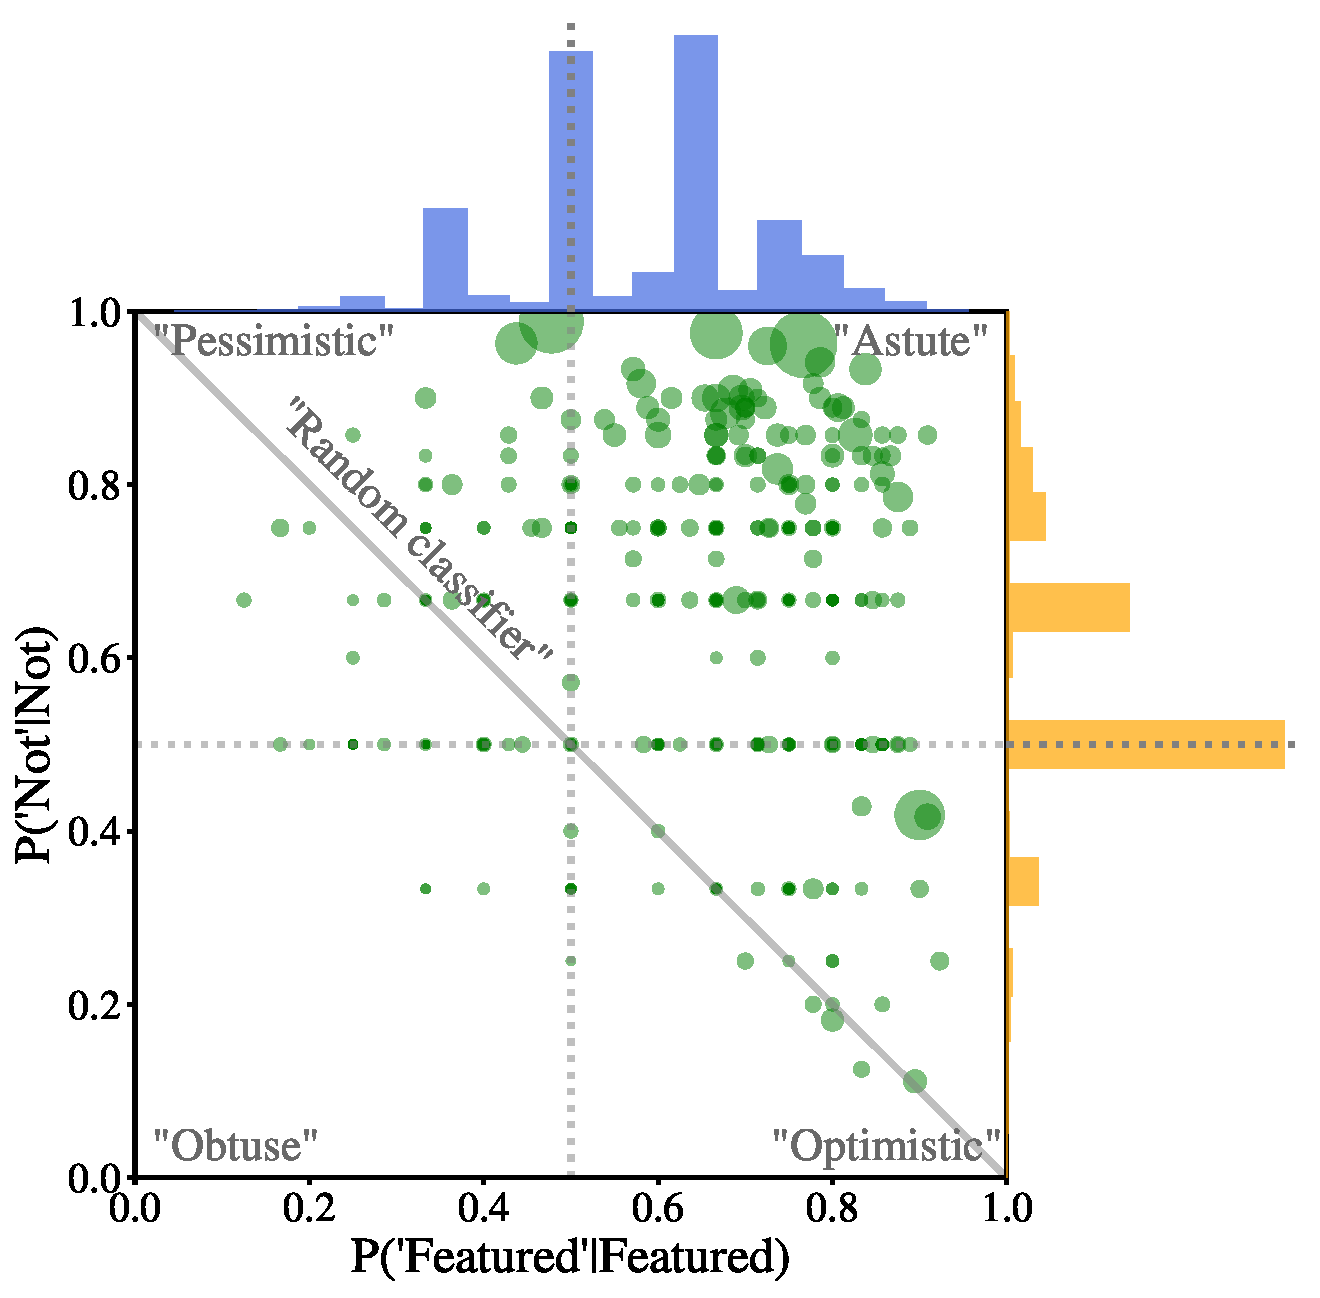
\includegraphics[width=3.45in]{Figures/human_machine/f2.pdf}
\caption[Galaxy Zoo volunteer confusion matrices achieved through SWAP.]{Confusion matrices for 1000 randomly selected GZ2 volunteers after fiducial SWAP assessment. Circle size is proportional to the number of gold standard subjects each volunteer classified. The histograms on top and right represent the distribution of each component of the confusion matrix for all volunteers.  A quarter of GZ2 volunteers are ``Astute"; \replaced{they are adept at correctly identifying both~\feat~and~\notfeat~subjects.}{they correctly identify both \feat~and \notfeat~subjects more than 50\% of the time.} The peaks at 0.5 in both distributions are due primarily to volunteers who see only one training image: only half of their confusion matrix is updated. \label{fig: volunteer training}}
\end{figure}


%%%-------------------------------------------------------
%%%  FIGURE:   SUBJECT POSTERIOR PROBABILITIES
%%%-------------------------------------------------------
\begin{figure}[t!] 
\centering
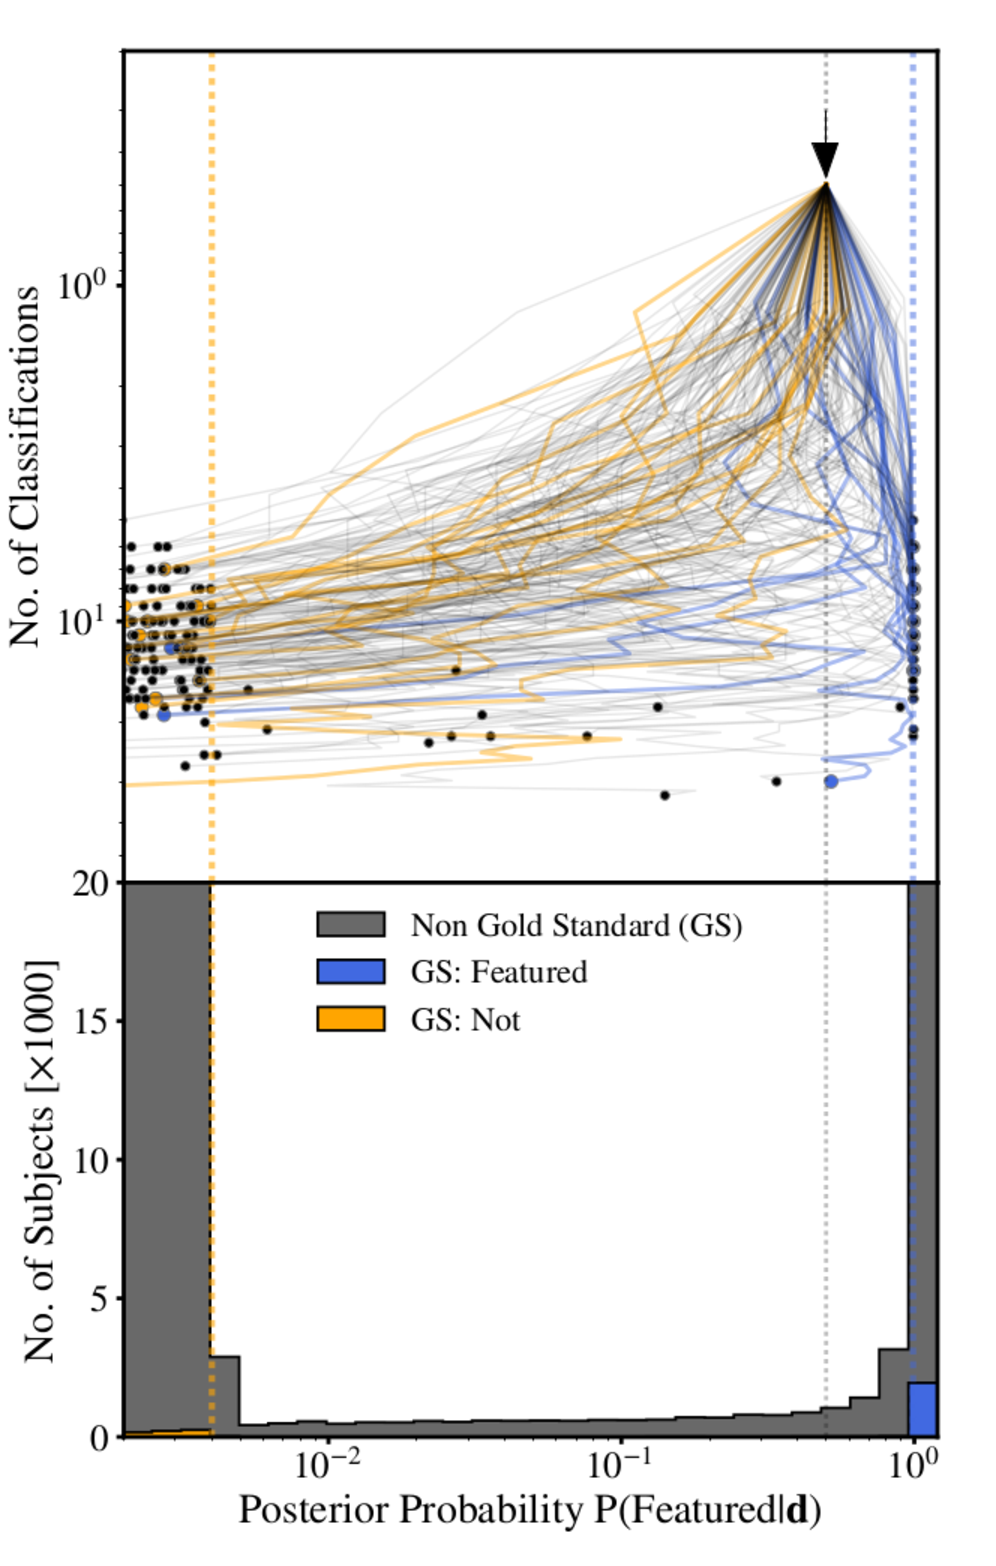
\includegraphics[width=3.25in]{Figures/human_machine/f12.pdf}
\caption[Galaxy posterior probabilities achieved through SWAP.]{Posterior probabilities for GZ2 subjects.  The top panel depicts the probability trajectories of 200 randomly selected GZ2 subjects. All subjects begin with a prior of 0.5 denoted by the arrow. Each subject's probability is nudged back and forth with each volunteer classification. From left to right the dotted vertical lines show the \notfeat~threshold, prior probability, and \feat~threshold. Different colours denote different types of subjects. The bottom panel shows the distribution in probability for all GZ2 subjects by the end of our simulation, where the y axis is truncated to show detail.  \label{fig: subject probabilities}}
\end{figure}

We create a gold standard sample by selecting 3496 SDSS galaxies representative 
of the relative abundance of T-Types, a numerical index of a galaxy's stage along 
the Hubble sequence, at $z\sim0$ by considering galaxies that overlap 
with the~\cite{NairAbraham2010} catalogue, a collection of $\sim$14K galaxies 
classified by eye into T-Types. 
\replaced{Expert classifications were obtained}
{We generate expert labels for these galaxies that are consistent with the labels we defined for GZ2 classifications. These are obtained} 
through the Zooniverse platform\footnote{The Project Builder template facility can be found at \url{http://www.zooniverse.org/lab.}}  
from 15 professional astronomers, including members of the Galaxy Zoo science team. 
 The question posed was identical to the original \added{top-level} GZ2 question 
and at least five experts classified each galaxy. 
Votes are aggregated and a simple majority provides an expert label for each subject. 
\added{This ensures that our expert labels are defined in exactly the same manner as the labels we assign the rest of the GZ2 sample.}
Our final dataset consists of the GZ2 classifications made 
by those volunteers who classify at least one of these gold standard subjects. 
We thus retain for our simulation 12,686,170 classifications from 30,894 unique volunteers. 
When running SWAP, classifications of gold standard subjects are always processed first. 



%%%-------------------------------------------------------
%%%  FIGURE:    SWAP FIDUCIAL RUN
%%%-------------------------------------------------------
\begin{figure}[t!]
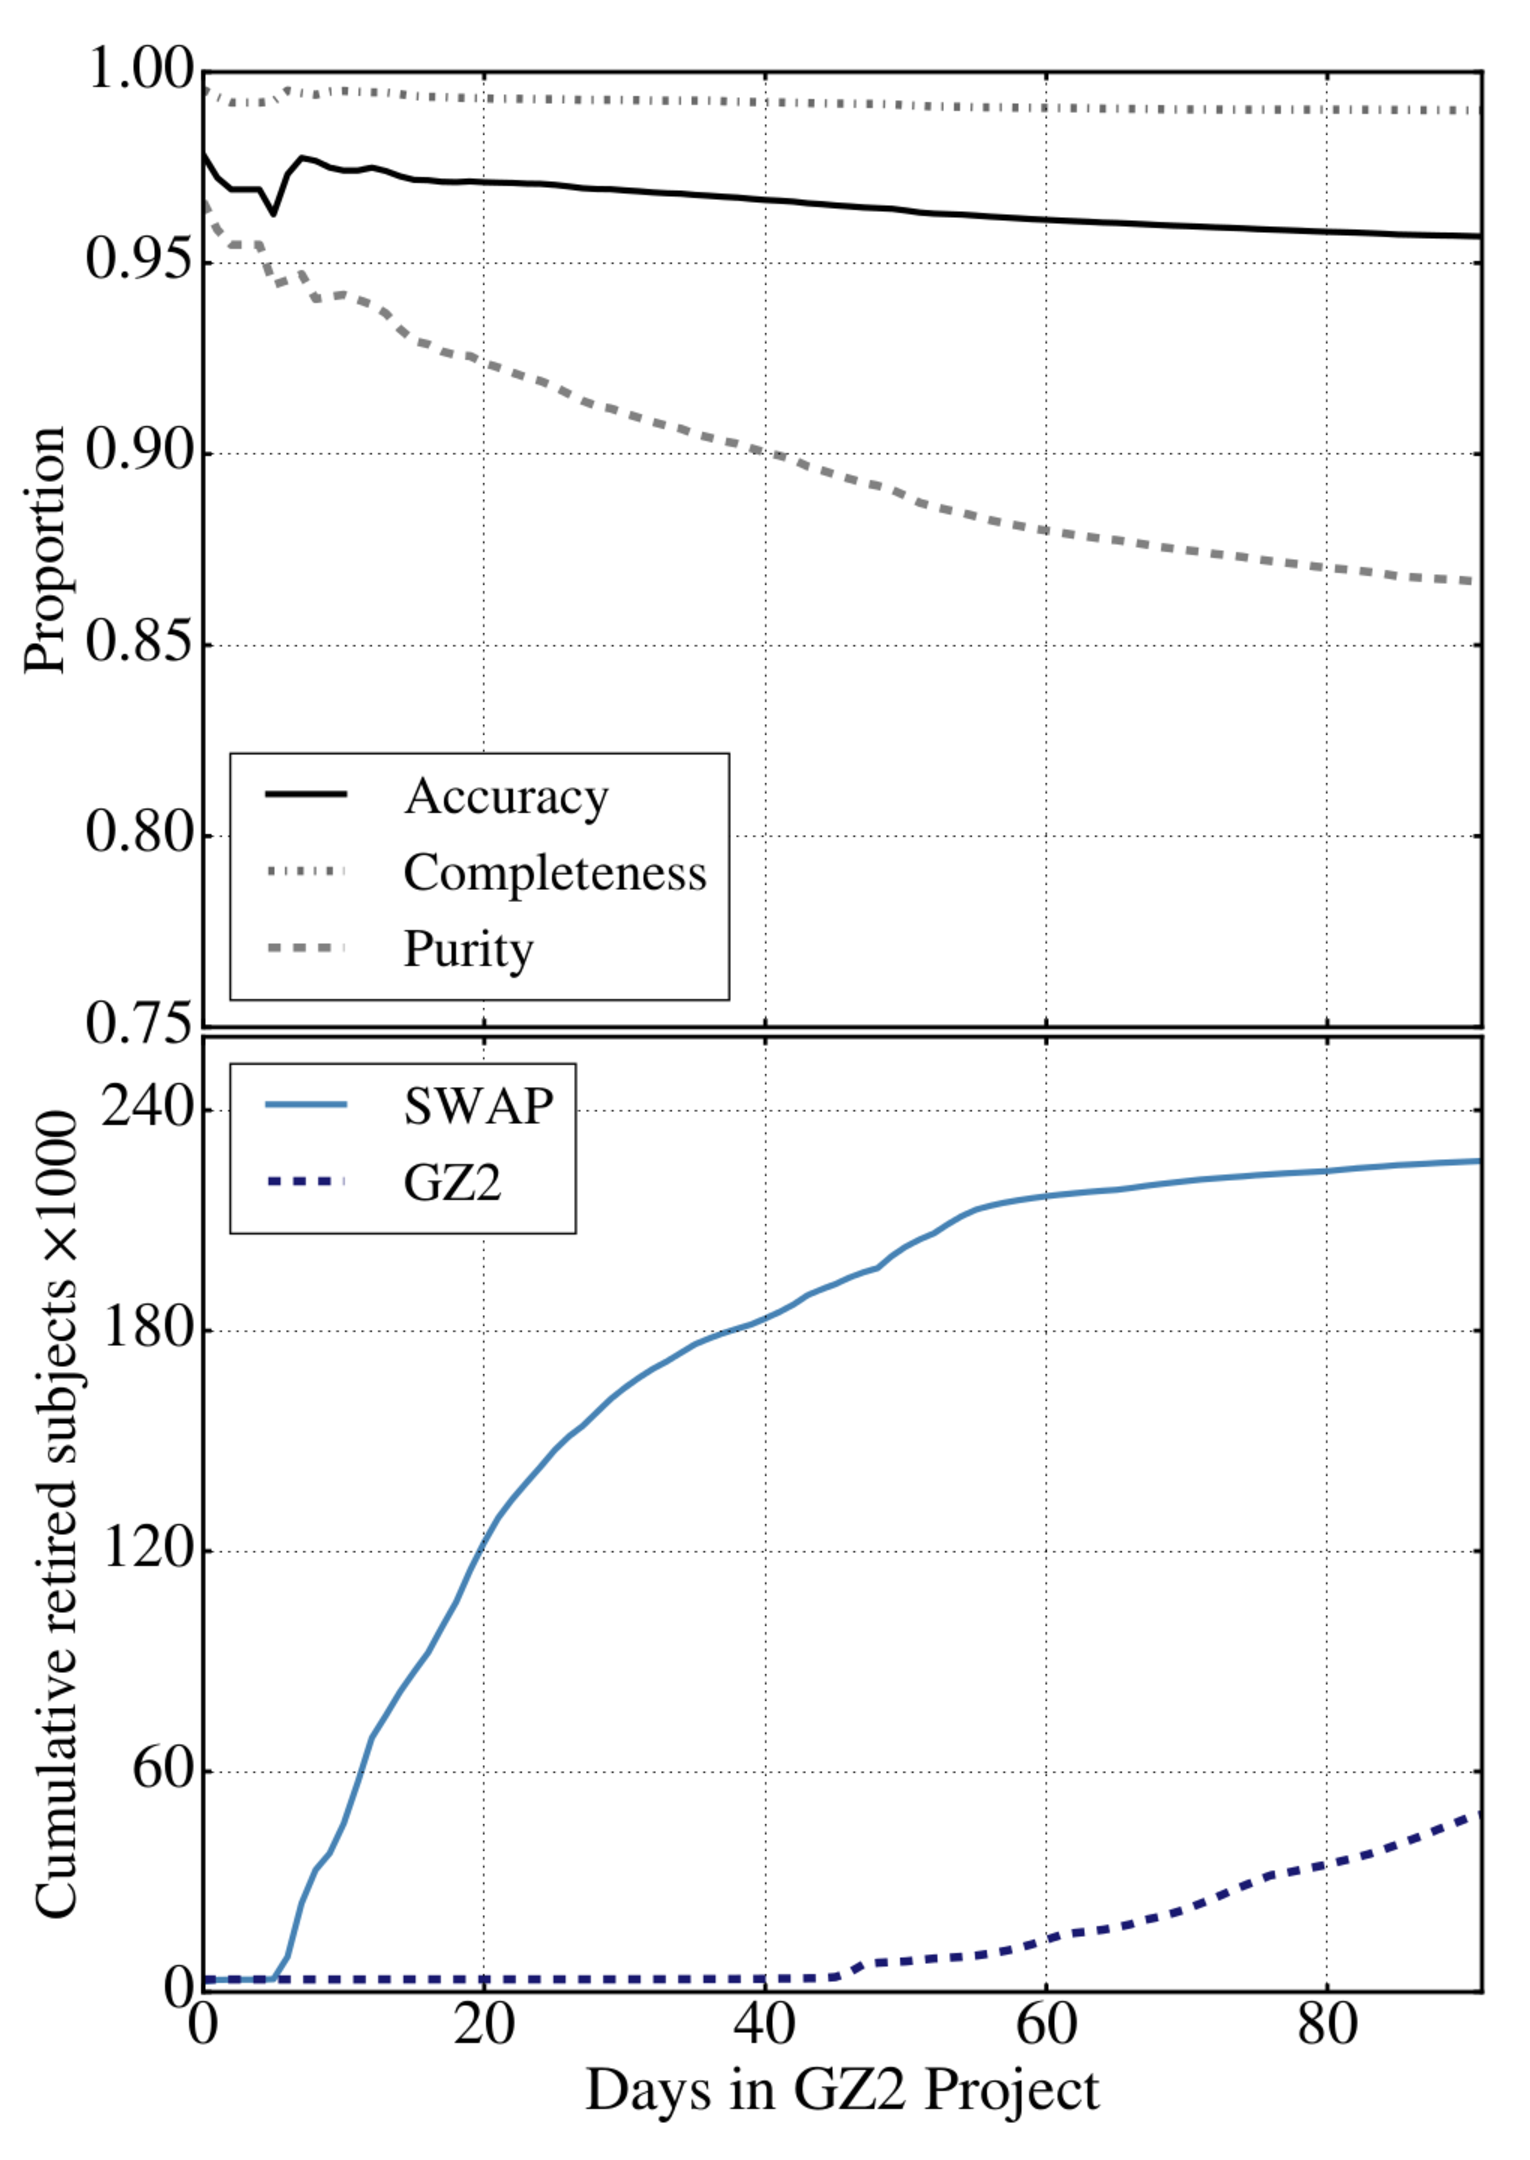
\includegraphics[width=3.35in]{Figures/human_machine/f3.pdf}
\caption[SWAP performance on Galaxy Zoo visual classifications.]{Fiducial SWAP simulation demonstrates a factor of 4-5 increase in the rate of subject retirement as a function of GZ2 project time (bottom panel, light blue) compared with the original GZ2 project (dashed dark blue). After 92 days, SWAP retires over 225K subjects, while GZ2 retires $\sim$48K.  The top panel displays the quality metrics (greys). These are calculated by comparing SWAP-assigned labels to~\raw~labels (Section~\ref{sec: data}) for the subject sample retired by that day of the simulation. Thus, on the final day, SWAP retires 226,124 subjects with 95.7\% accuracy,  and with completeness and purity of~\feat~subjects at 99\% and 86.7\% respectively. The decrease in purity as a function of time is due, in part, to the fact that more difficult to classify subjects are retired later in the simulation. 
\label{fig: fiducial run}}
\end{figure}



%%----------------------------------------------------------------------------------------------------------------------------------------------------
%%   Subsection:    		SWAP only (FIDUCIAL RUN)
%%----------------------------------------------------------------------------------------------------------------------------------------------------
\subsection{Fiducial SWAP simulation}\label{sec: fiducial}

Before we run a simulation, a number of SWAP parameters must be chosen: 
 the initial confusion matrix for each volunteer's agent, \added{(\Pf, \Pn)};
the subject prior probability, \added{\p}; and the retirement thresholds, \added{\tf~and \tn}. 
For our fiducial  simulation, we initialize all confusion matrices at (0.5, 0.5), 
and set the subject prior probability, \p~$= 0.5$. 
We set the~\feat~threshold, \tf, i.e., the minimum probability for a subject to be retired as~\feat, to $0.99$. Similarly, we set the~\notfeat~threshold, \tn~$= 0.004$. 
In Appendix~\ref{sec: tweaking swap} 
we show that varying these parameters has only a small affect on the SWAP output. 
To simulate a live project, we run SWAP on a time step of $\Delta t = 1$ day, 
during which SWAP processes all volunteer classifications with timestamps 
within that range. This is performed for three months worth of GZ2 classification data. 


Figure~\ref{fig: volunteer training} (adapted from Figure 4 of~\citealt{Marshall2016})
demonstrates the volunteer assessment we achieve, and shows confusion matrices 
 for 1000 randomly selected volunteers. The circle size is proportional to the number of 
gold standard subjects each volunteer classified. 
The histograms represent the distribution of each component
of the confusion matrix for all volunteers.
 Nearly 25\% of volunteers are considered ``Astute"  indicating
they \replaced{are generally good at correctly identifying both~\feat~and~\notfeat~subjects.}{correctly identify both \feat~and \notfeat~subjects more than 50\% of the time. 
Furthermore, as long as a volunteer's confusion matrix is different from random, 
they provide useful information to the project.}
The spikes at $0.5$ in the histograms are due to volunteers who see only one 
gold standard subject (i.e.,~\feat), leaving their probability in the 
other (\notfeat) unchanged.
Additionally, 4\% of volunteers have a confusion matrix of (0.5, 0.5) indicating these 
volunteers classified two gold standard subjects of the same type, one correctly and 
one incorrectly. 

\added{
Figure~\ref{fig: subject probabilities} (adapted from Figure 5 of \citealt{Marshall2016}) 
demonstrates how subject posterior probabilities are updated with each classification. 
The arrow in the top panel denotes the prior probability, \p~$=0.5$. 
With each classification, that prior is updated into a posterior probability creating a trajectory through probability space for each subject. 
The blue and orange lines show the trajectories of a random sample of \feat~and 
\notfeat~subjects from our gold standard sample, while the black lines show the 
trajectories of a random sample of GZ2 subjects that were not part of the 
gold standard  sample. The similarly coloured vertical dashed lines correspond to the
 retirement thresholds, \tf~and \tn. The lower panel shows the full distribution of 
GZ2 subject posteriors at the end of our simulation, where the y-axis has been truncated to show detail. An overwhelming majority of subjects cross one of these retirement thresholds. }

Our goal is to increase the efficiency of galaxy classification. We therefore
 use as a metric the cumulative number of retired subjects
as a function of the original GZ2 project time.
We define a subject as GZ2-retired once it achieves at least 30 volunteer votes, 
encompassing 98.6\% of GZ2 subjects.
In contrast, a subject is considered SWAP-retired once its posterior 
probability crosses either of the retirement thresholds defined above. 


However, it is important not to prioritize efficiency at the expense of quality. 
We thus also consider the metrics of accuracy, 
purity and completeness as a function of GZ2 project time.  
These are defined as follows: accuracy is the number of correctly
identified subjects divided by the total number retired; completeness is the number of 
correctly identified~\feat~subjects divided by the number of actual~\feat~retired; 
and purity is the number of correctly identified~\feat~subjects divided by 
the number of subjects retired as~\feat. Thus, a complete sample has no false
negatives whereas a pure sample has no false positives. 
We compute these metrics by comparing the SWAP-assigned labels of the cumulatively 
retired subject set to the~\raw~labels for each day of the simulation. 
For example, by Day 20, SWAP retires 120K subjects with 96\% accuracy,
 99.7\% completeness, and 92\% purity. 

Figure \ref{fig: fiducial run} and Table~\ref{tab: summary} detail the results of 
our fiducial SWAP simulation compared to the original GZ2 project. 
The bottom panel shows the cumulative number of retired subjects as a function of 
GZ2 project time. By the end of our simulation, GZ2 (dashed dark blue)
 retires $\sim$50K subjects while SWAP (solid light blue) retires 226,124 subjects.  
We thus classify 80\% of the entire GZ2 sample in three months. 
\replaced{The original GZ2 project took approximately one year to classify as many subjects, 
representing a factor of four increase in the classification rate. }
{Here we consider the number of classifications logged each day and not the length 
of time spent on a single classification.  Under the assumption that collapsing the 
GZ2 decision tree to a single question would not have decreased the number of 
classifications  collected each day during the GZ2 project, processing volunteer classifications 
through SWAP presents a striking increase in classification efficiency.}
The top panel of Figure~\ref{fig: fiducial run} demonstrates the quality of 
those classifications as a function of time and establishes that our full 
SWAP-retired sample is 95.7\% accurate, 99\% complete, and 86.7\% pure. 
\added{We discuss these small discrepancies in Section~\ref{sec: swap gz2 disagree}.}

%%%-------------------------------------------------------
%%%  FIGURE:   SWAP vote distributions
%%%-------------------------------------------------------
\begin{figure}[t!] 
\centering
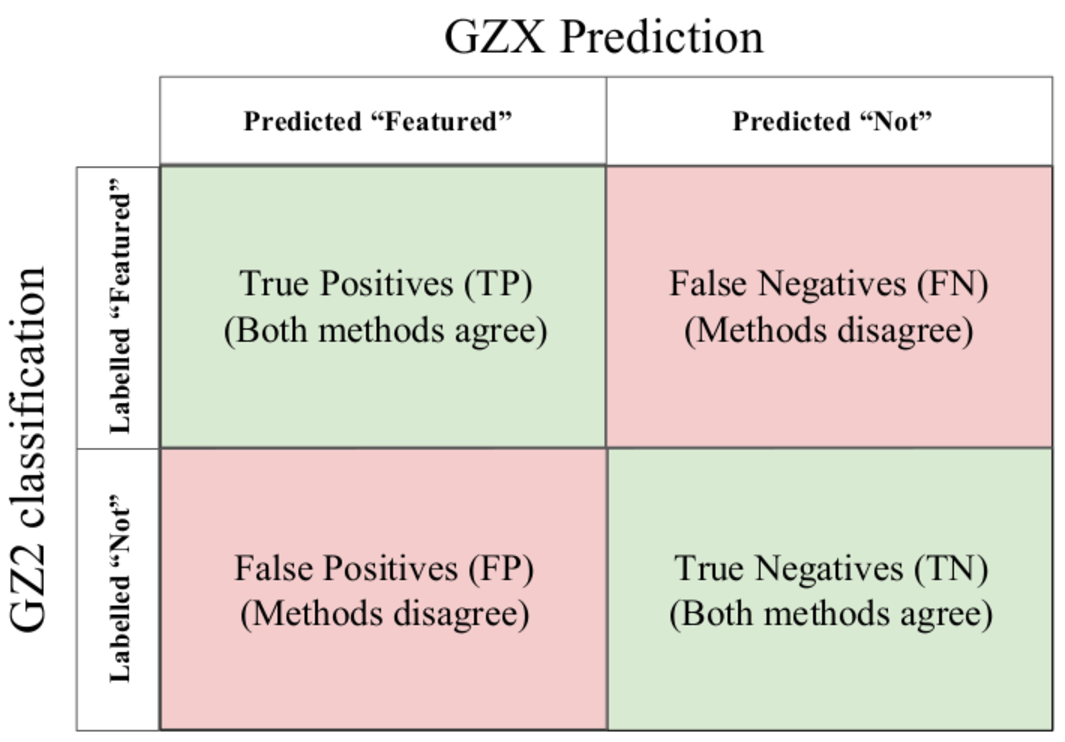
\includegraphics[width=3.5in]{Figures/human_machine/f4.pdf}
\caption[SWAP volunteer weighting mechanism reduces human effort for classification]{SWAP's volunteer-weighting mechanism provides a factor of three reduction in the human effort required to retire GZ2 subjects. The filled histograms show the number of volunteer classifications per subject achieved from our simulation of GZ2 data broken down by class label, where the solid black line is the total. The dashed histograms are results from our toy model in which we simulate volunteers with fixed confusion matrices, effectively disengaging SWAP's volunteer-weighting mechanism. These broad distributions require $\sim$3 times more classifications per subject to reach the same retirement thresholds.} 
\label{fig: swap vote distributions}
\end{figure}

\added{\subsection{Reducing human effort}}
\replaced{
There is also a reduction in the human effort required to perform this classification task.
  Figure~\ref{fig: swap vote distributions} shows the distribution of the number 
of volunteer classifications per subject achieved through SWAP (light blue) 
and GZ2 (dark blue) for the 226K subjects retired in our fiducial run. 
GZ2's distribution peaks at $\sim$45 indicating that, on average,
45 unique volunteers classify each subject. On the other hand, SWAP's
distribution peaks around 9 classifications per subject. 
Furthermore, subjects that are `easy' to classify (i.e.,~\feat) require
even fewer classifications to reach strong consensus. 
More precisely, SWAP processes $2.3 \times 10^6$ volunteer 
classifications while GZ2 records $\sim$$10^7$ for the same subject set. 
SWAP reduces human effort by more than a factor of four. }
{The SWAP algorithm effectively weights volunteers according to how many gold 
standard subjects they correctly identify. This mechanism provides a reduction 
in the amount of human effort required to perform this classification task. 
To see this, we consider a toy model wherein we simulate volunteers with fixed 
confusion matrices. We simulate 1000 \feat~subjects and 1000 \notfeat~subjects 
each with prior, \p~$ = 0.5$. We simulate 100 volunteer agents all with the same 
fixed confusion matrix of (0.63, 0.65), where these values are computed as the 
average \Pf~and \Pn~from our assessment of real volunteers, excluding the spikes at 0.5. 
We generate volunteer classifications based on this confusion matrix 
(i.e., volunteers will correctly identify \feat~subjects 63\% of the time) 
and update the subject's posterior probability with each classification. 
We track how many classifications are required for each subject's posterior to 
cross either the \feat~or \notfeat~retirement thresholds. } 

\added{The results are presented in Figure~\ref{fig: swap vote distributions}. 
The filled blue and orange histograms show the number of volunteer classifications 
per subject achieved from our simulation of GZ2 data, where volunteer agent confusion
 matrices are those from Figure~\ref{fig: volunteer training}. The dashed blue 
and orange distributions are the results from our toy model. When SWAP accounts 
for volunteer skill, most subjects are retired with between 6 and 15 votes, with 
a median of 9 votes. In contrast, when every volunteer is given equal weighting, 
subjects require 16 to 45 votes with a median of 30 votes before crossing one of 
the retirement thresholds. Thus the volunteer weighting scheme embedded in 
SWAP can reduce the amount of human effort required to retire subjects by a factor of three.}

\added{This reduction will be, in part, a function of the number of gold standard 
subjects each volunteer sees.  Our gold standard sample was chosen to be 
representative of morphology rather than evenly distributed among GZ2 volunteers. 
We thus find that half of our volunteers classify only one or two gold standard subjects. 
That we achieve a factor of three reduction when only half of our volunteer pool 
has seen $\ge 2$ gold standard subjects suggests that an additional reduction of
  human effort is possible with more extensive volunteer training.}

%%%-------------------------------------------------------
%%%  FIGURE:   SWAP failures
%%%-------------------------------------------------------
\begin{figure}[t!]
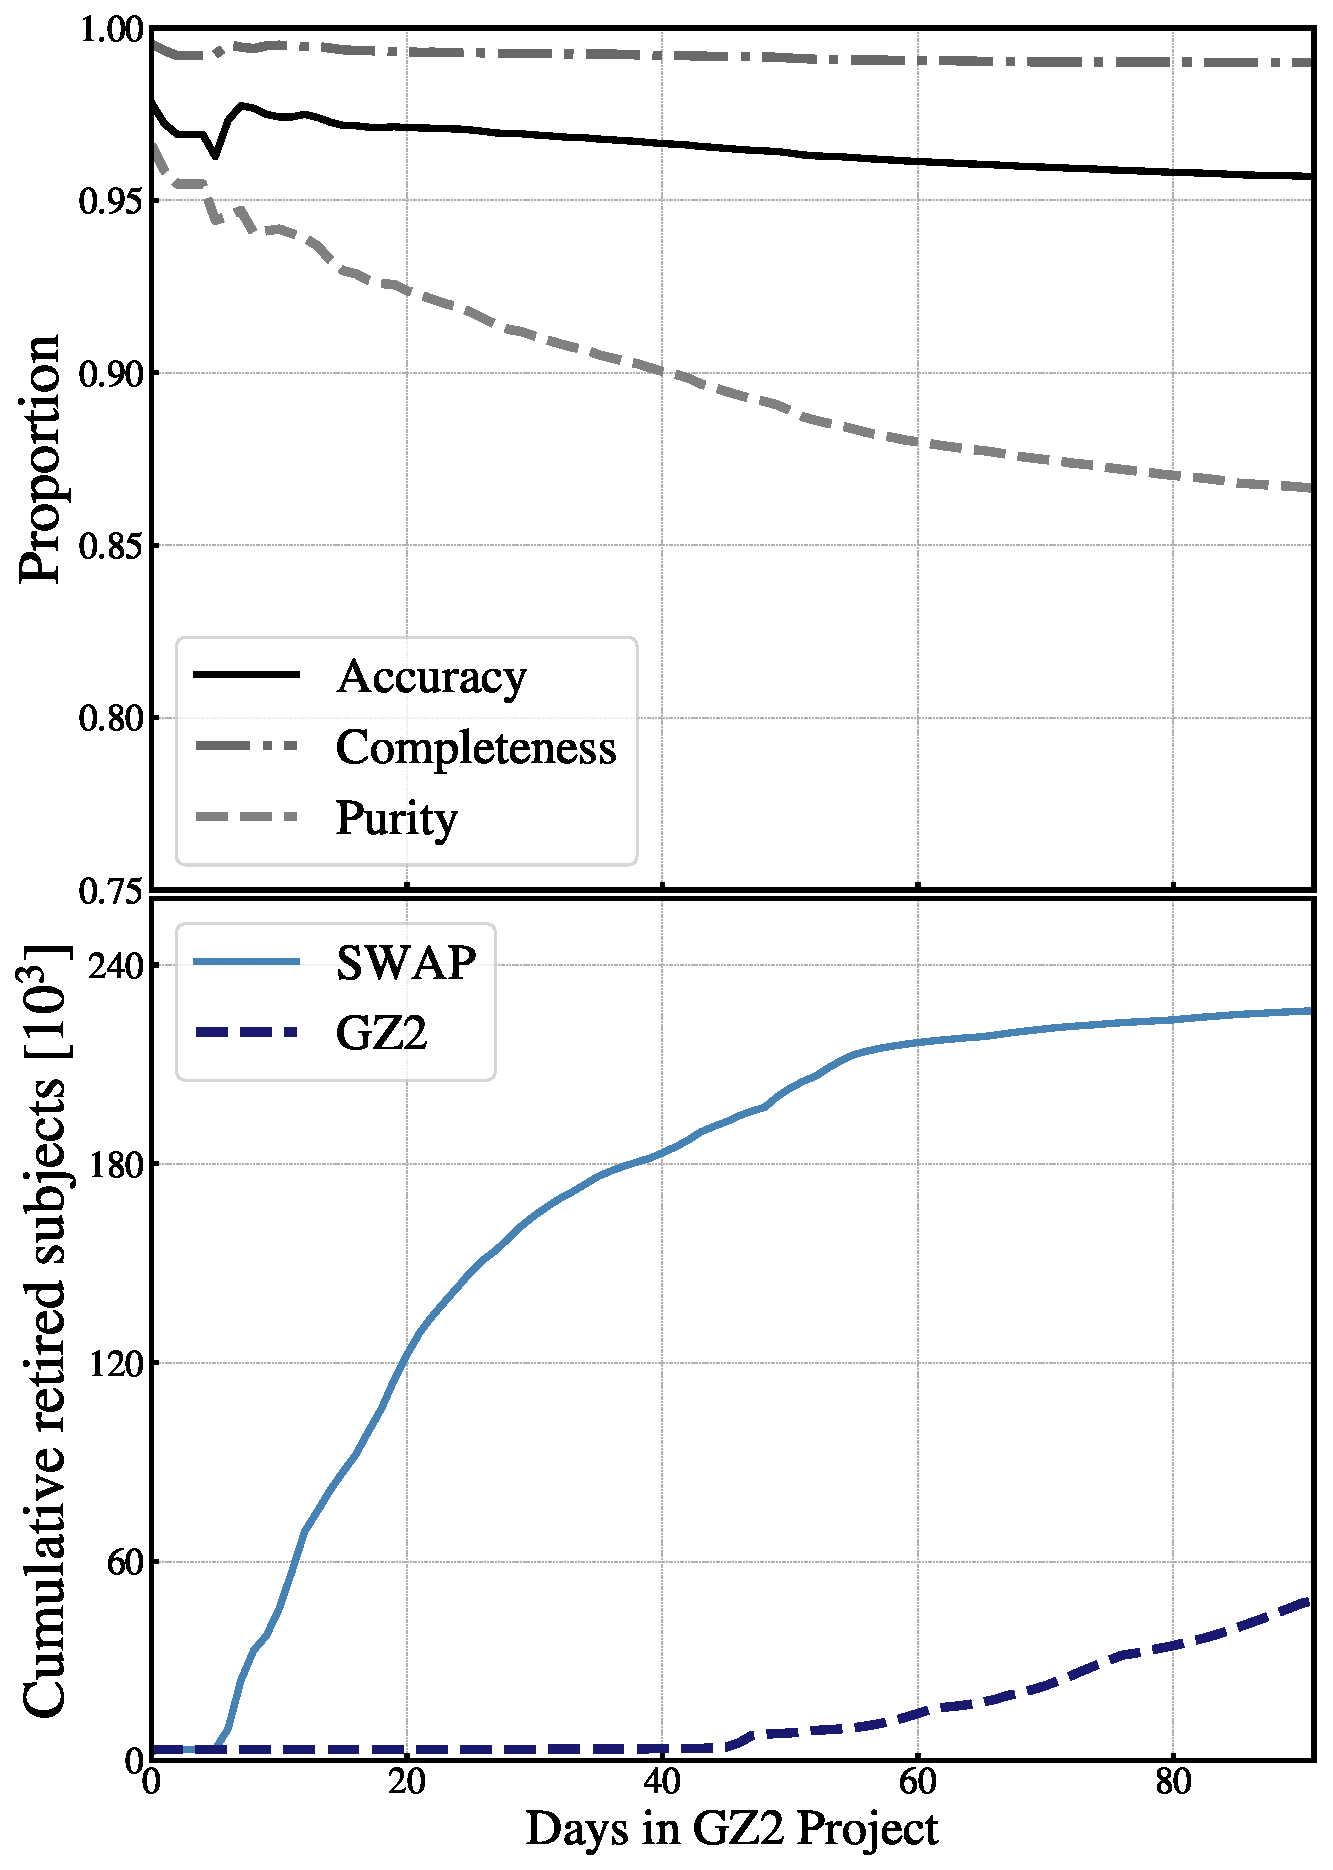
\includegraphics[width=3.5in]{Figures/human_machine/f5.pdf}
\caption[$f_{featured}$ distribution of SWAP misclassifications]{Distribution of GZ2 \ffeat+\fstar~vote fractions for subjects correctly identified by SWAP (dotted grey), along with those identified as false positives (solid purple), and false negatives (dashed teal). 
The false positives and false negatives are scaled by factors of 10 and 100 respectively for easier comparison. From Section~\ref{sec: data}, subjects with values $> 0.5$ are defined as~\feat, however, the teal distribution indicates that SWAP labels them as~\notfeat. This is not a flaw of SWAP: 68.9\% of incorrectly identified subjects have $0.4 \le $~\ffeat +\fstar~$ \le 0.6$ suggesting that~\raw~labels are simply too uncertain. The overlap between the false positives and negatives is due to subjects that are exactly 50-50; by default these are labelled~\notfeat. \label{fig: SWAP sucks}}
\end{figure}


\subsection{Disagreements between SWAP and GZ2}\label{sec: swap gz2 disagree}

Galaxy Zoo's strength comes from the consensus of dozens of volunteers voting on each subject. 
Processing votes with SWAP reduces the number of classifications to reach consensus. 
Though we typically recover the~\raw~label, SWAP disagrees about 5\% of the time. 
We thus examine the false positives (subjects SWAP labels as~\feat~but~\raw~labels as~\notfeat) and false negatives (subjects SWAP labels as~\notfeat~but~\raw~labels as~\feat).
\added{We explore these subjects in redshift, magnitude, physical size, and concentration. We find no correlation with any of these variables, suggesting that, at least for this galaxy sample, the reliability of morphology depends on factors that are not captured by these coarse measurements.
This is perhaps unsurprising since GZ2 subjects were selected from the larger GZ1 sample to be the brightest, largest and nearest galaxies:  precisely those subjects most accessible for visual classification. }

\replaced{We find the majority of these disagreements are due to uncertainties in 
the~\raw~label.}{Instead we consider the stochastic nature of GZ2 vote fractions, which can be estimated as binomial. Let success be a response of ``smooth'' and failure be any other response. The $68\%$ confidence interval on a subject with \fsmooth~$=0.5$ is then $(0.42, 0.57)$ assuming 40 classifications, each with a probability of 0.5.}
Figure~\ref{fig: SWAP sucks} shows the distribution of~\ffeat+\fstar~for the false positives (solid purple), and the false negatives (dashed teal) compared to the
 subjects where SWAP and GZ2 agree (dotted grey).  
Recall that if this value is greater than 0.5, the subject is labelled~\feat.  
The majority of \replaced{incorrectly labelled}{disagreements between SWAP and GZ2 are for} 
subjects that have $0.4 <$~\ffeat+\fstar~$< 0.6$. \replaced{indicating that 
the GZ2 raw vote fractions are simply too uncertain to provide high quality labels.}{It is thus unsurprising that SWAP and GZ2 disagree most within the approximate confidence interval of our selected GZ2 threshold.} 
We note that the distribution overlap between false positives and false negatives is due to subjects that do not have a majority;
these are labelled~\notfeat~by default. 


Two other effects contribute to the disagreement between SWAP and GZ2. 
First, as the number of classifications used to retire a galaxy decreases, the 
likelihood of misclassification by random chance increases. 
Second, disagreement arises due to expert-level volunteers whose confusion 
matrices are close to 1.0. These volunteers are essentially more 
strongly weighted, allowing that subject's posterior to cross a retirement threshold
in as few as two classifications. In rare cases, despite training, some expert-level 
volunteers get it wrong \added{compared to the gold-standard labels}. These issues can be mitigated by requiring each subject reach 
a minimum number of classifications in addition to its probability crossing a
retirement threshold, thus combining the best qualities of GZ2 and SWAP. 


\subsection{Summary}

%In Appendix~\ref{sec: tweaking swap}, we find that varying the initial SWAP 
%parameters from the fiducial values does not substantially change the results 
%presented here. The largest influence comes from choosing unrealistic subject 
%prior probabilities, which can mildly degrade the quality of the resulting classifications. 
%More importantly, none of these effects significantly alters our human and machine integration in Section~\ref{sec: results}. 


We demonstrate a factor of four or more increase in 
classification efficiency while maintaining 95\% accuracy, nearly perfect 
completeness of~\feat~subjects, and with a purity that can be controlled by careful 
selection of input parameters to be better than 90\% (see Appendix~\ref{sec: tweaking swap}).
Exploring those subjects wherein SWAP and GZ2 disagree, we conclude that 
the majority of this disagreement stems from \replaced{uncertainty in}{the stochastic nature of}~\raw~labels.
We now turn our focus towards incorporating a machine
classifier utilizing these SWAP-retired subjects as a training sample. 




\section{Stuff from the appendix -- fold into the main text}

\textbf{Initial agent confusion matrix.} 
In our fiducial simulation each volunteer was assigned an agent whose confusion matrix was
initialized at $(0.5, 0.5)$, which presumes that volunteers are no better than random classifiers.  
We perform two simulations wherein we initialize agent confusion matrices as $(0.4, 0.4)$, 
slightly obtuse volunteers; and $(0.6, 0.6)$, slightly astute volunteers, with everything else remaining constant.  
Results of these simulations compared to the fiducial run are shown in the left panel of
Figure~\ref{fig: tweak swap}. We find that SWAP is largely insensitive to the 
initial confusion matrix  both in terms of the subject retirement rate and classification quality.  



%% -------------------------------------------------------------------------------
%%   FIGURE:  SWAP --  CONFUSION MATRIX & PRIOR 
%% -------------------------------------------------------------------------------
\begin{figure*}[th]
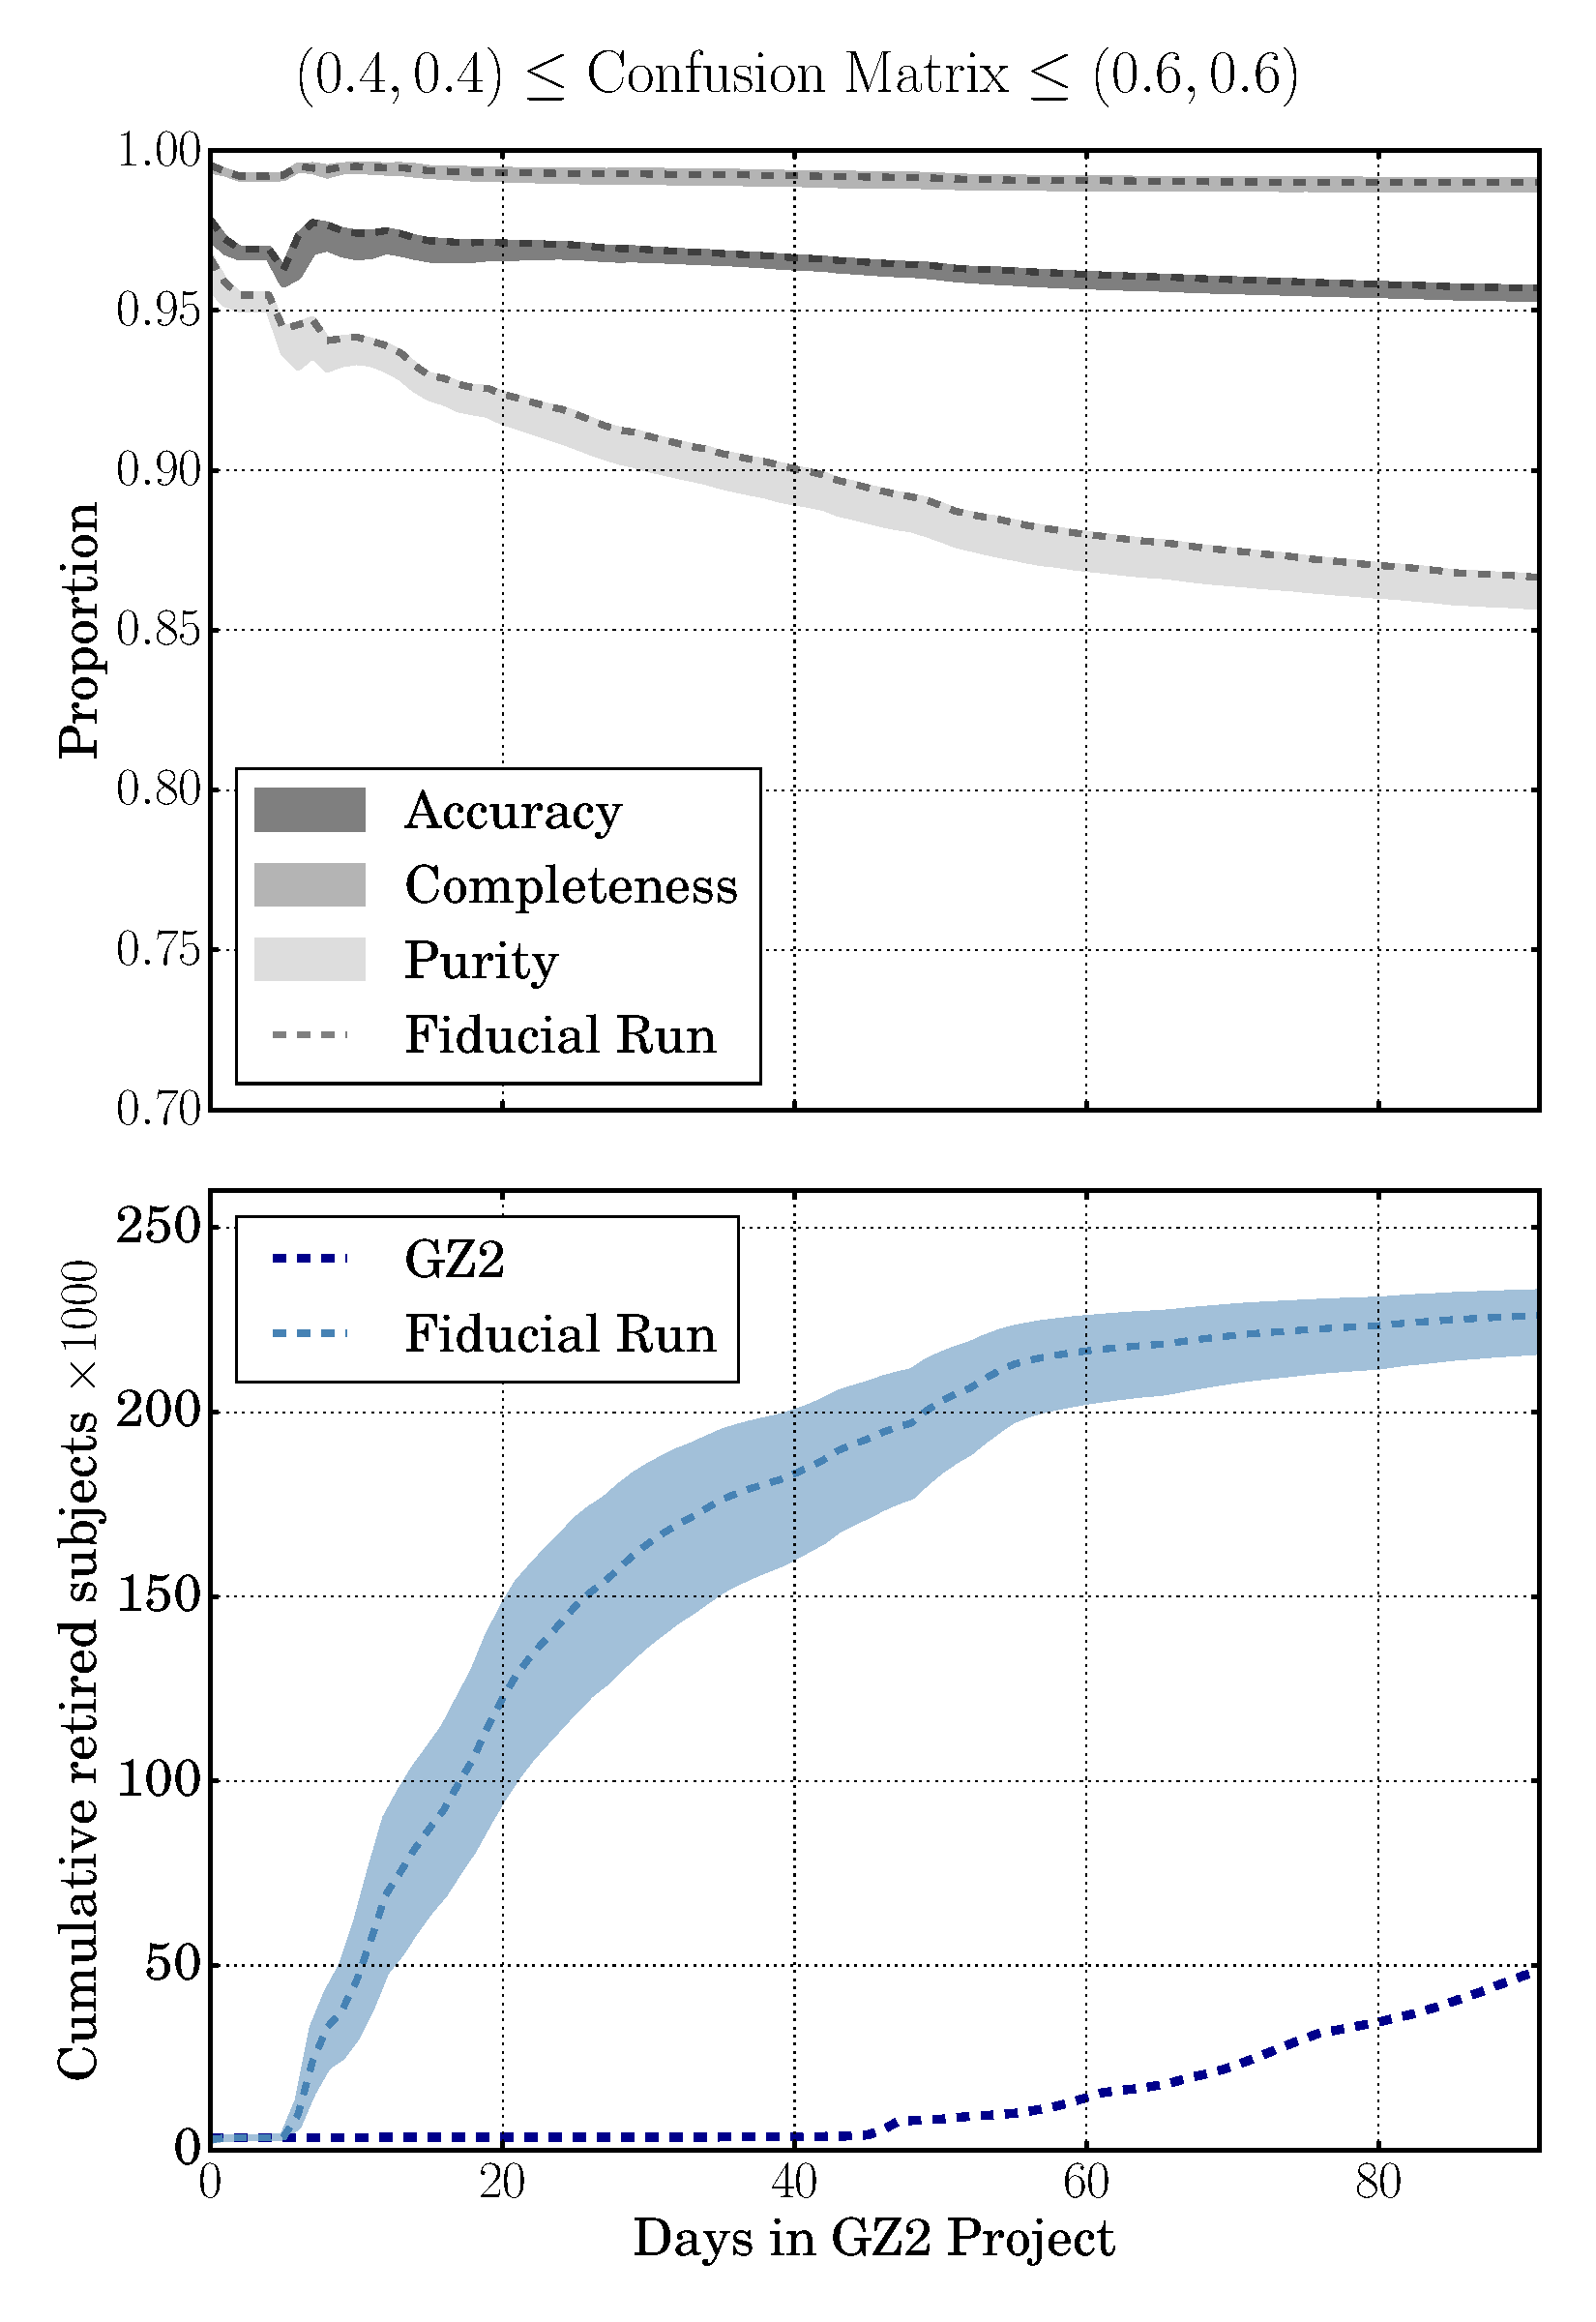
\includegraphics[width=2.9in]{Figures/human_machine/A1a.pdf}
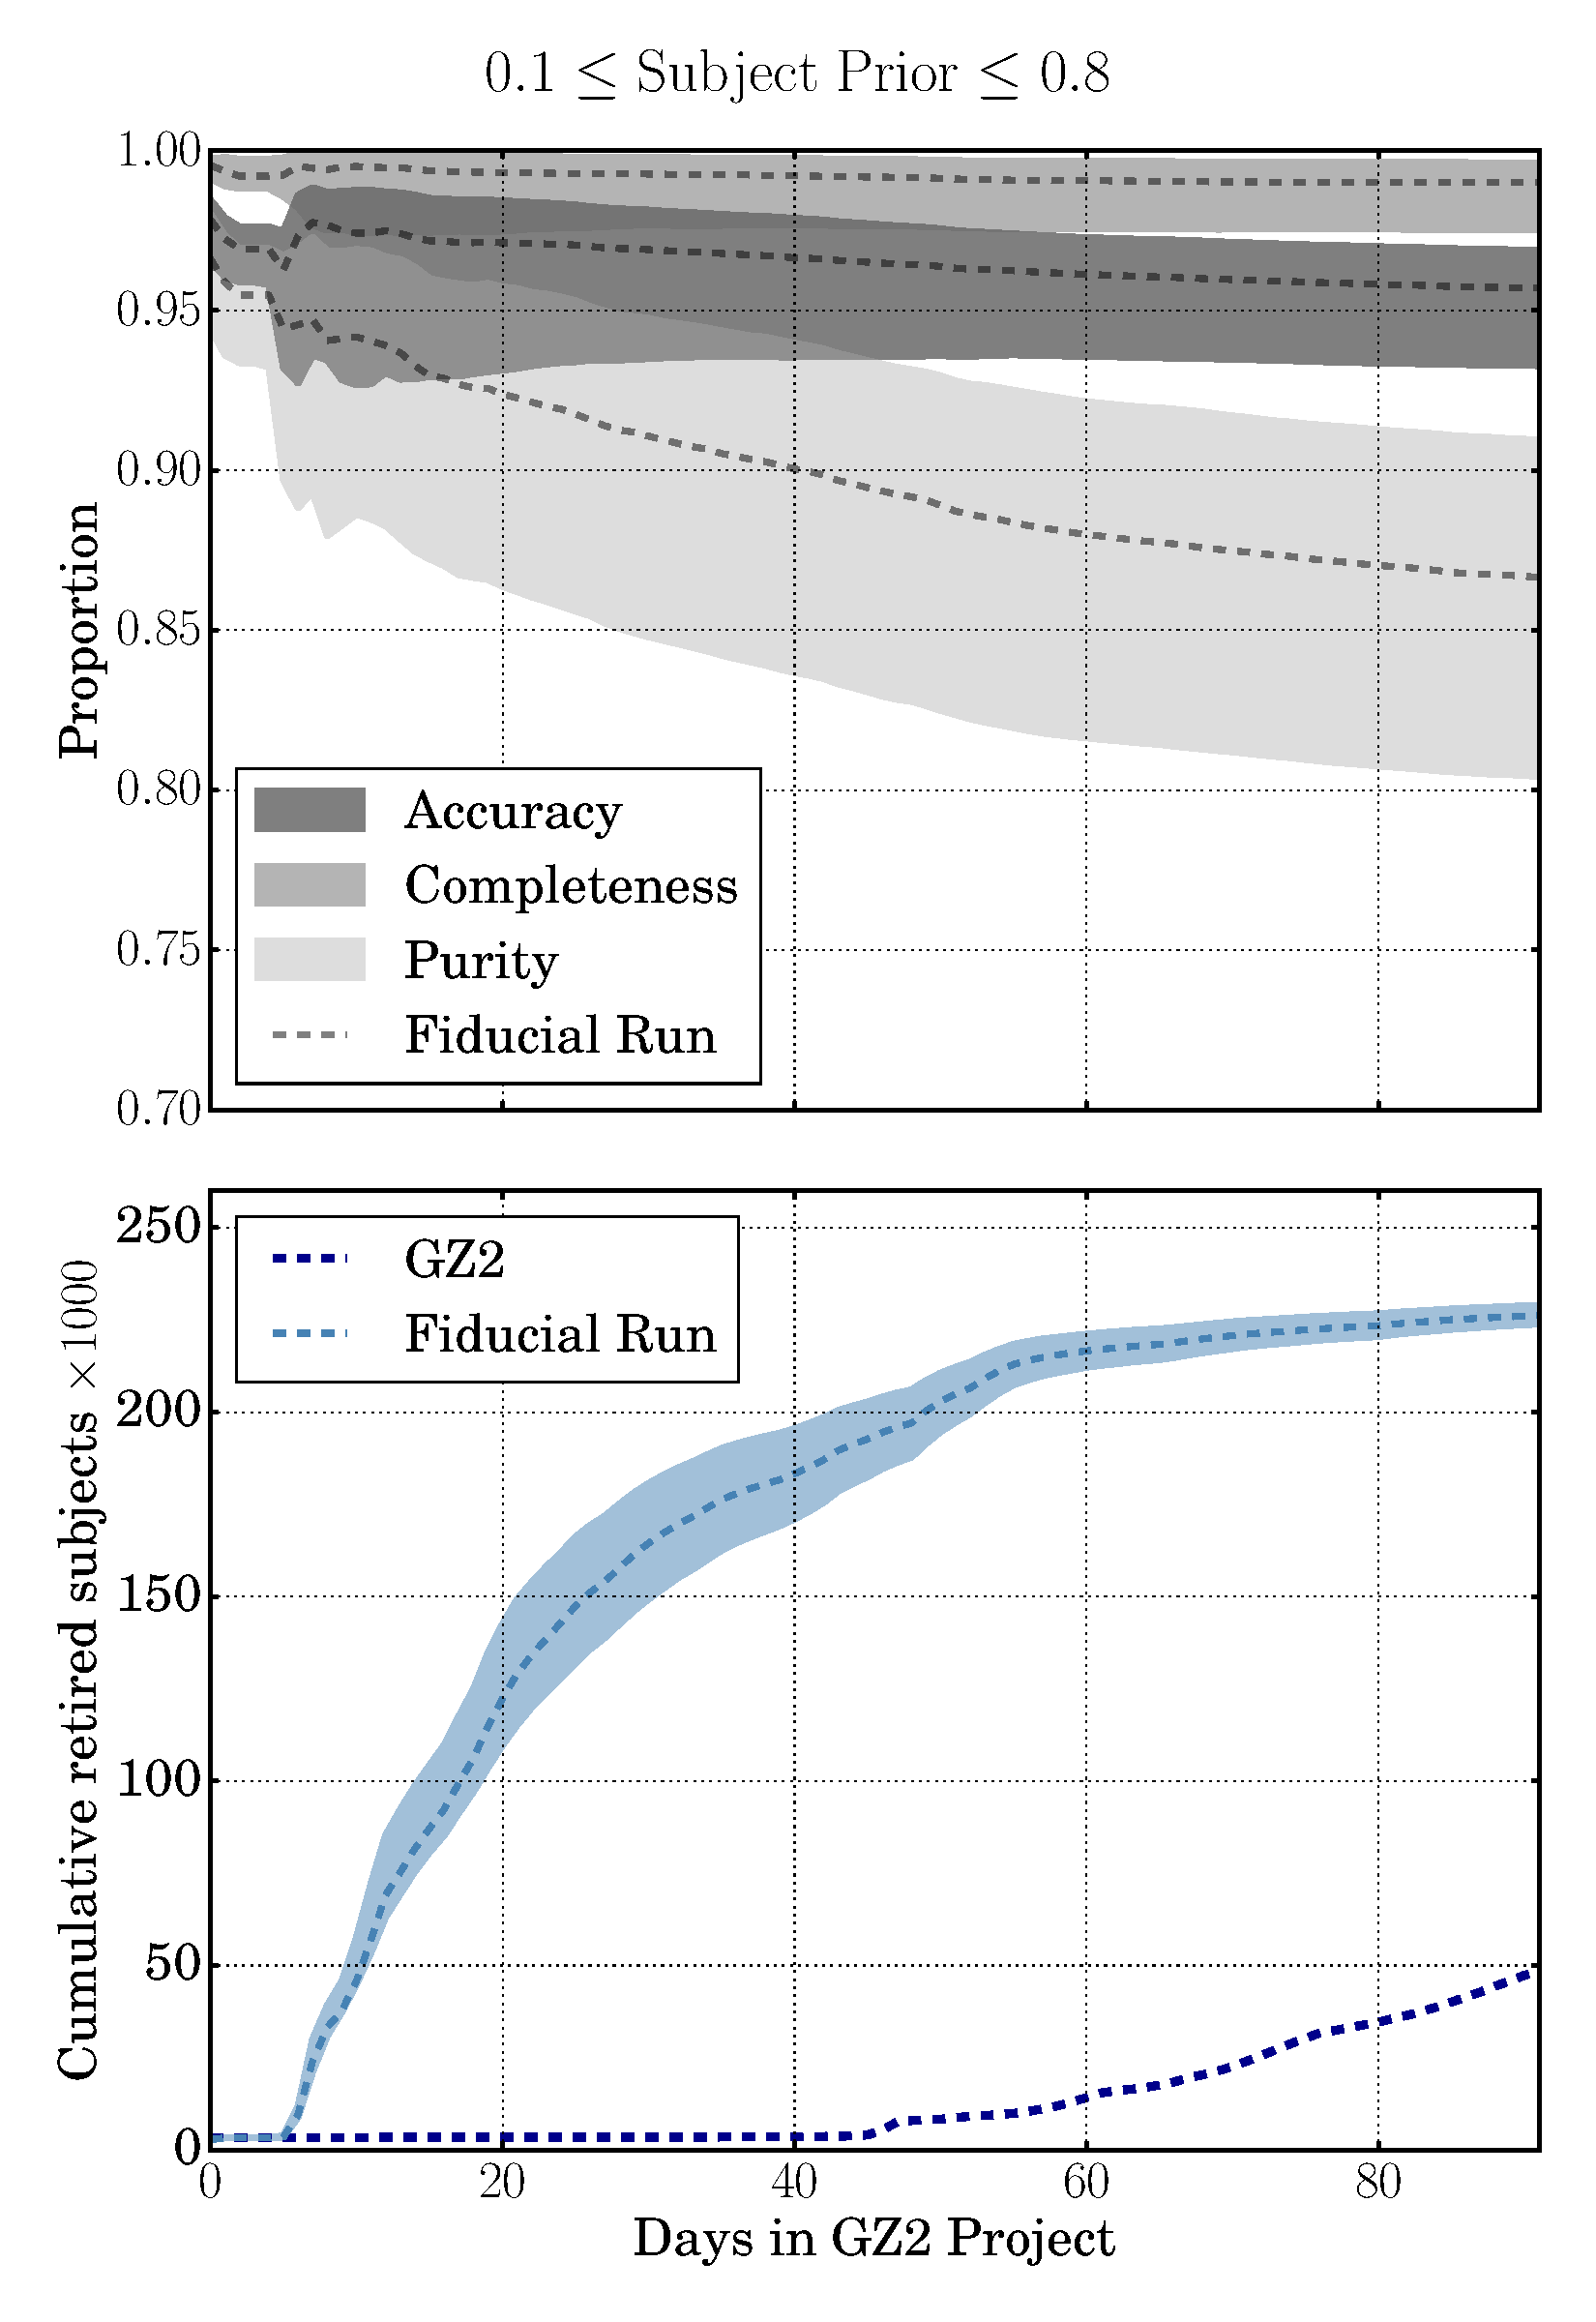
\includegraphics[width=2.9in]{Figures/human_machine/A1b.pdf}
\caption{SWAP performance does not dramatically change even with a range of input parameters (shaded regions) as compared to the fiducial run of Section~\ref{sec: fiducial} (dashed lines).  \textit{Left.} The quality (top) and retirement rate (bottom) when the confusion matrix is initialized as (0.4, 0.4) and (0.6, 0.6), with all other input parameters remaining constant. \textit{Right.} Same as the left panel but allowing the subject prior probability, \p $= 0.2, 0.35$ and $0.8$. Changing the confusion matrix has little impact on the quality of the labels but varies the total number of subjects retired. In contrast, changing the subject prior is more likely to affect the classification quality rather than the total number of subjects retired. \label{fig: tweak swap}}
\end{figure*}

We retire $\sim$$225$K$\pm3.5\%$ subjects as shown by the light blue shaded region in the bottom
left panel of Figure~\ref{fig: tweak swap}, where the dashed blue line denotes the fiducial run. 
Predictably, when the confusion matrix probabilities are low, we retire fewer subjects 
than when these probabilities are high for a given period of time. 
This is easy to understand since it takes longer for volunteers to become astute 
classifiers when they are initially given values denoting them as obtuse. 
Regardless, most volunteers become astute classifiers by the end of the simulation. 
The top left panel demonstrates our usual quality metrics as computed in Section \ref{sec: fiducial}.
The dashed lines again denote the fiducial run. 
We maintain $\sim$$95\%$ accuracy, $99\%$ completeness, and $\sim$$84\%$ purity;
 and no metric changes by $> 2\%$ regardless of initial confusion matrix values.  
 
This spread is due to three effects: 
1) subjects can receive an alternate SWAP label in different simulations, 
2) subjects can be retired in a different order, and 
3) the set of retired subjects is not guaranteed to be common to all runs. 
We find SWAP to be highly consistent: 
more than 99\% of retired subjects are the same among all simulations, 
and, of these, 99\% receive the same label.  Instead we find that the order in which 
subjects are retired changes between runs. 
When the confusion matrix is low, subjects take longer to classify compared to the fiducial run 
(i.e., they retire on a later date in GZ2 project time). 
Likewise, subjects retire sooner when the confusion matrix is high. 
This can cause quality metrics to vary since they are calculated on a day to day basis. 
These effects each contribute less than one per cent variation and thus we see a 
high level of consistency between simulations. 

Of interest, perhaps, is that the quality metrics for these simulations are not symmetric 
about the fiducial run. However, in the Bayesian framework of SWAP, an agent with 
confusion matrix (0.4, 0.4) contributes as much information as an agent with confusion matrix (0.6, 0.6).
The quality metrics computed are thus within a per cent of each other.
In either case, we find that initializing agents at (0.5, 0.5) provides optimal performance 
for the `training' we simulate with our current approach. Further assessment would 
require a live project with real-time training and feedback. 


%%%-------------------------------------------------------
%%%  FIGURE:   MORPH PARAMS & SWAP THRESHOLDS
%%%-------------------------------------------------------
\begin{figure*}[t!]
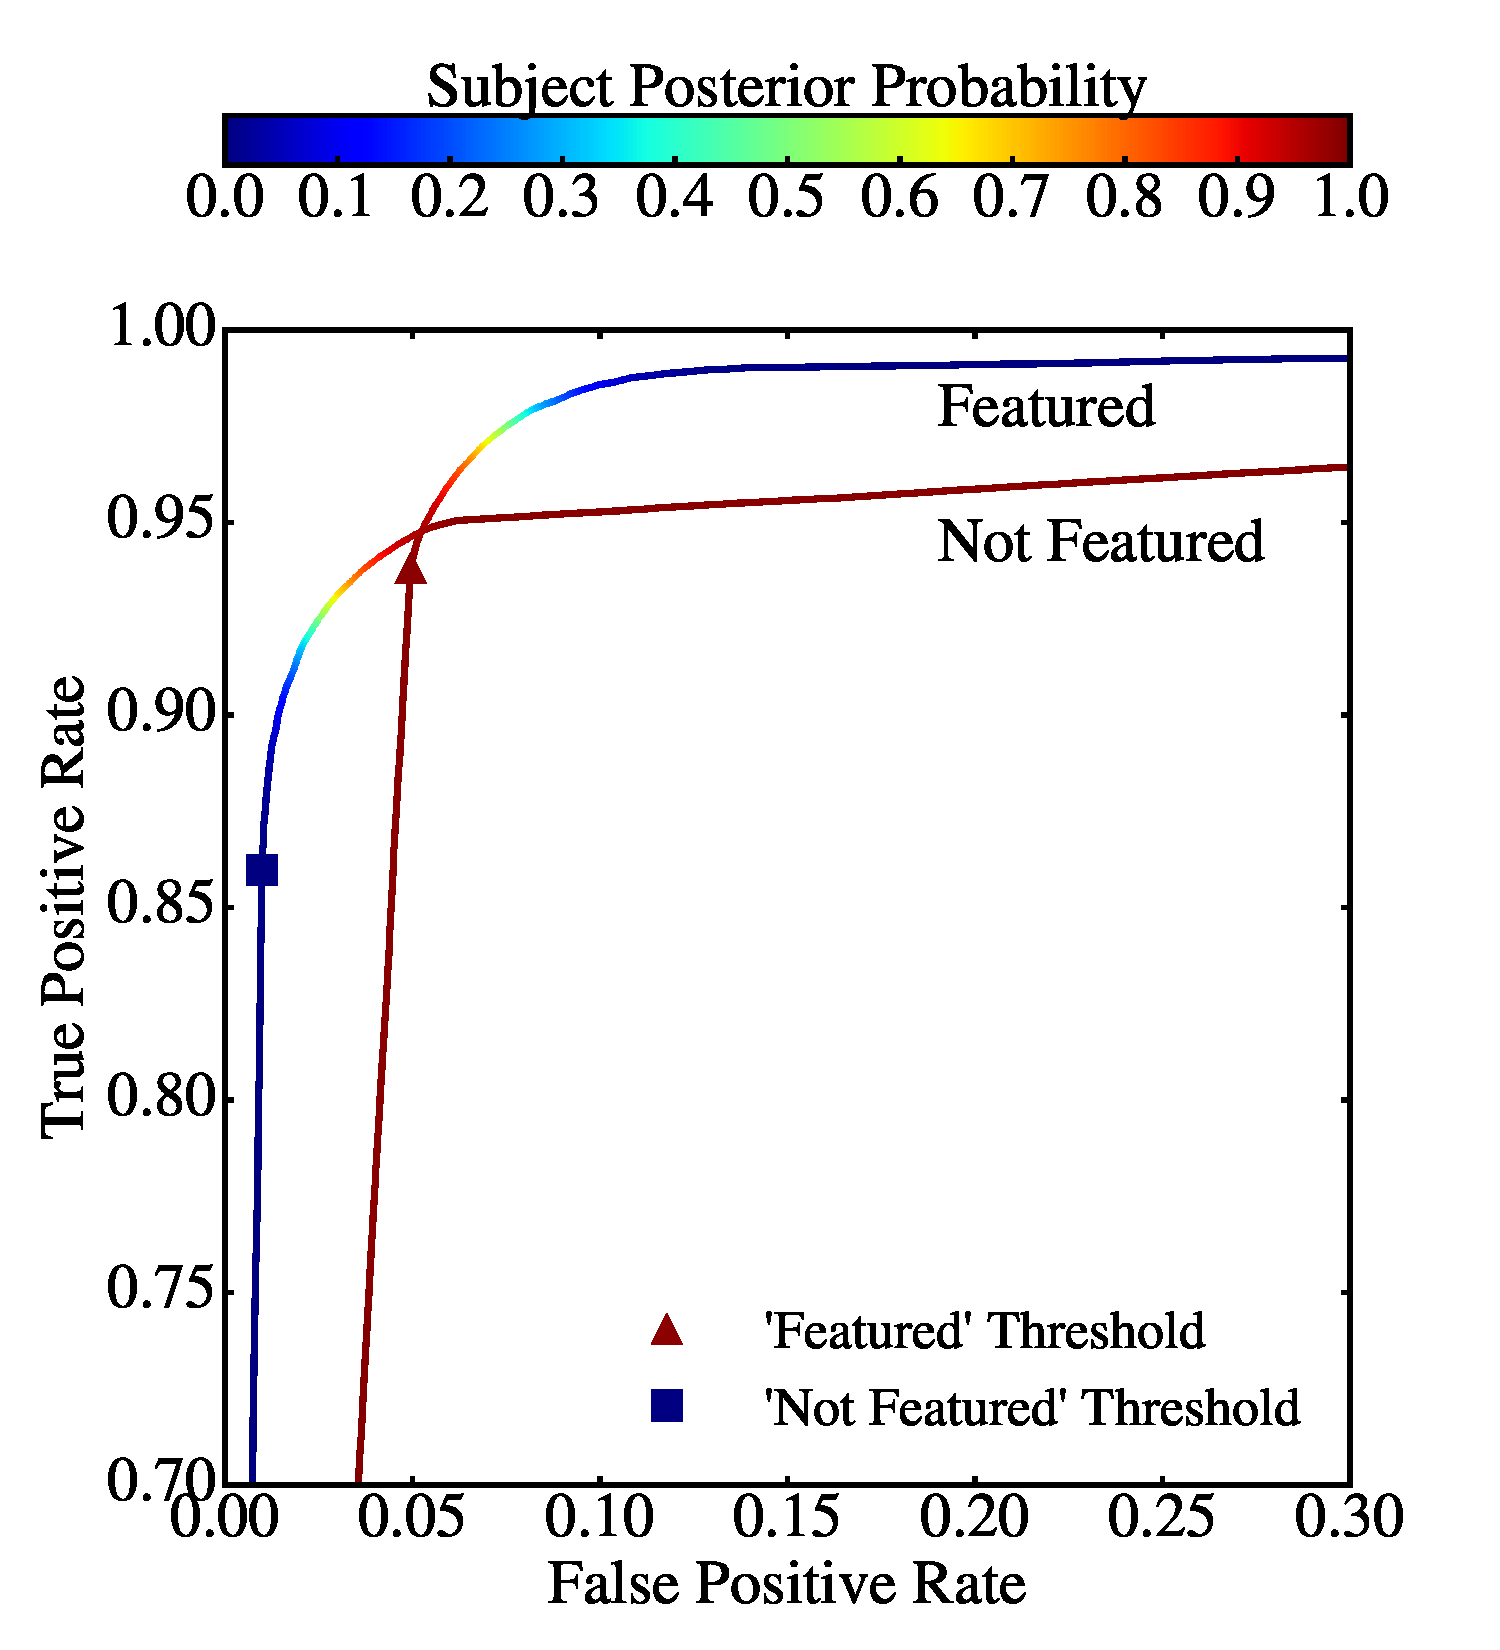
\includegraphics[width=3.08in]{Figures/human_machine/A2a.pdf}
\caption{\textit{Left.} Identifying~\feat~subjects is independent of identifying~\notfeat~subjects.  Both ROC curves use all subjects processed by SWAP where the score used to create the ROC curve is simply each subject's achieved posterior probability. The Featured curve demonstrates how well we identify~\feat~subjects with a threshold of 0.99, while the Not Featured curve demonstrates how well we identify~\notfeat~subjects with a threshold of 0.004. Typically, best performance is achieved by the score associated with the upper-left-most part of the curve. Our~\feat~threshold is nearly optimal, while our~\notfeat~threshold could be improved since the blue square is not as close to the upper left hand corner as other possible values of the subject posterior. \textit{Right.} Relation between measured morphology diagnostics for more than 280K SDSS galaxies. Most of these galaxies are processed through SWAP, receiving a posterior probability that estimates how likely each is to be~\feat~or~\notfeat.}
\label{fig: morph thresh}
\end{figure*}


\textbf{Subject prior probability,~\p.}
The prior probability assigned to each subject is an educated guess of 
the frequency of that characteristic in the scope of the data at hand. 
For galaxy morphologies, this number should be an estimate of the probability
of observing a desired feature (bar, disk, ring, etc.). In our case, 
we desire simply to find galaxies that are~\feat; however, this is dependent 
on mass, redshift, physical size, etc. The original GZ2 sample was selected
primarily on magnitude and redshift.  As there was no cut on galaxy size
(with the exception that each galaxy be larger than the SDSS PSF), the sample
includes a large range of  masses and sizes. Designating a single prior is not clear-cut; 
we thus explore how various~\p~values effect the SWAP outcome.

We run simulations allowing~\p~to take values 0.2, 0.35, and 0.8 
and compare these to the fiducial run, with everything else remaining constant.
The results are shown in the right panels of Figure~\ref{fig: tweak swap}. 
We again find that SWAP is consistent in terms of subject retirement which varies by only 1\%. 
However, as can be seen in the top panel, the variation in our quality metrics is 
more pronounced. 
Firstly, though we retire nearly the same number of subjects over the course
of each simulation, they are less consistent than our previous runs. That is, 
only 95\% of retired subjects are common to all simulations. Secondly, of those that are 
common, only 94\% receive the same label from SWAP indicating that changing the prior 
is more likely to produce a different label for a given subject than changing the initial 
agent confusion matrix. Finally, there is also a larger spread for the day on which a subject 
is retired as compared to the fiducial run. These trends all contribute to a broader 
spread in accuracy, completeness, and purity as a function of project time.
We stress, however, that although more substantial than the previous comparison, 
these variations are all within $\pm5\%$. 

We can understand these variations more intuitively by considering the following.
Recall that our retirement thresholds,~\tf~and~\tn, have not changed in these simulations. 
When~\p~is small, the subject's probability is already closer to~\tn~in probability space, 
and thus more subjects are classified as~\notfeat~compared to the fiducial run.
Similarly, when~\p~is large, some of these same subjects can instead be classified
as~\feat~because~\p~is already closer to~\tf. Obviously, both outcomes cannot be correct. 
We find that the simulation with~\p~= 0.8 performs the worst of any run; 
this is a direct reflection of the fact that this prior is not suitable for this question or this dataset. 
 Indeed, the best performance is achieved when~\p = 0.35.  This reflects the 
distribution of~\feat~subjects as determined by~\raw~labels and is more characteristic
of the expected proportion of~\feat~galaxies in the local universe.
As a value far from the correct value can have a significant impact on the classification
quality, it is important to choose a prior wisely.
 


\textbf{Retirement thresholds, \tf~and~\tn.}
Retirement thresholds are directly related to the time that a subject will spend
in SWAP before retirement.  If we lower~\tf~(and/or raise~\tn), more subjects will be retired
compared to the fiducial run as each subject will have a smaller swath of probability space
in which to fluctuate before crossing one of these thresholds.
On the other hand, if we raise~\tf~(and/or lower~\tn), it will take longer for subjects
to cross one of these thresholds. This also increases the likelihood of some subjects 
never crossing either threshold, instead oscillating indefinitely through probability space.

What thresholds should one choose? To answer this question, we consider the left panel of
Figure~\ref{fig: morph thresh}, which depicts the receiver operating 
characteristic (ROC) curve for our fiducial simulation, an illustration of performance as a 
function of a threshold for a binary classifier. 
ROC curves display the true positive rate against the false positive rate for 
a discriminatory threshold or score with a perfect classifier achieving 100\% true positives
and no false positives. The value of the threshold optimal for predicting class labels would 
be that which allows the ROC curve to reach the upper-left-most point in the diagram. 
We have two thresholds to consider and thus we plot the curve twice: 
once under the assumption that ``true positives" denote correctly identified~\feat~subjects; 
and again under the assumption that ``true positives" instead denote correctly identified~\notfeat~subjects.  In both cases, the colour of the line corresponds to the 
subject posterior probability. We mark the location of~\tf~$=0.99$~and~\tn~$=0.004$
from our fiducial run with a red triangle and blue square respectively. 
 We see that~\tf~is nearly optimal but~\tn~could be improved upon.